\pagebreak
\section{Ai-je bien compris ? }
\begin{UPSTIactivite}
\UPSTIquestion{Sous chaque dispositif, indiquer s'il s'agit d'un actionneur, pré-actionneur ou un capteur. Pour les capteurs, précisez le type (analogique, numérique ou logique) : }

\begin{minipage}[b]{0.24\textwidth}
\centering
  Ventilateur industriel
  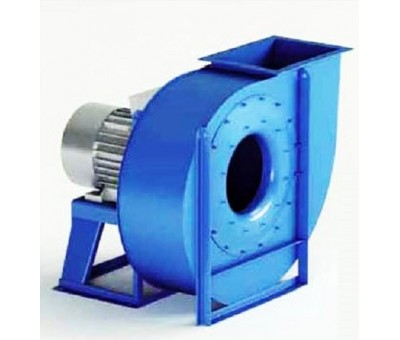
\includegraphics[width=\textwidth,height=.15\textheight,keepaspectratio]{images/ventilateurIndus}

  \UPSTIaCompleter{\large{Actionneur}}

\end{minipage}
\begin{minipage}[b]{0.24\textwidth}
\centering
  Sonde de pression
  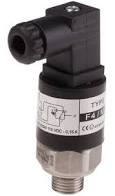
\includegraphics[width=\textwidth,height=.15\textheight,keepaspectratio]{images/sondePression}

  \UPSTIaCompleter{\large{Capteur analogique}}

\end{minipage}
\begin{minipage}[b]{0.24\textwidth}
\centering
  Electrovanne
  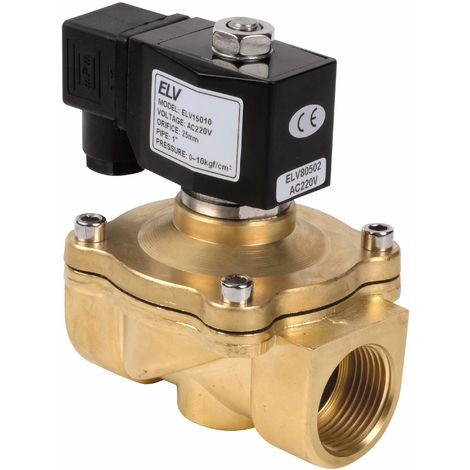
\includegraphics[width=\textwidth,height=.15\textheight,keepaspectratio]{images/electrovanne}

  \UPSTIaCompleter{\large{Actionneur}}

\end{minipage}
\begin{minipage}[b]{0.24\textwidth}
\centering
  Distributeur pneumatique
  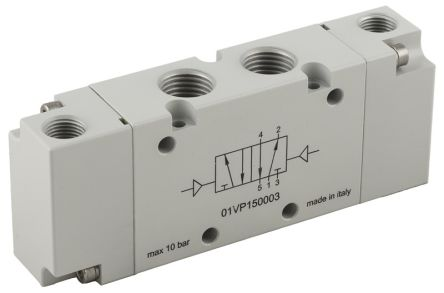
\includegraphics[width=\textwidth,height=.15\textheight,keepaspectratio]{images/distri_electroPneu}

  \UPSTIaCompleter{\large{Pré-actionneur}}

\end{minipage}

\vspace*{0.5cm}

\begin{minipage}[b]{0.24\textwidth}
\centering
  Résistance chauffante
  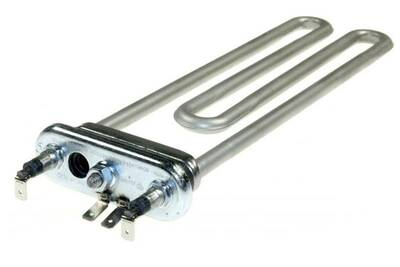
\includegraphics[width=\textwidth,height=.15\textheight,keepaspectratio]{images/resistanceChauffante}

  \UPSTIaCompleter{\large{Actionneur}}

\end{minipage}
\begin{minipage}[b]{0.24\textwidth}
\centering
  Détecteur de présence
  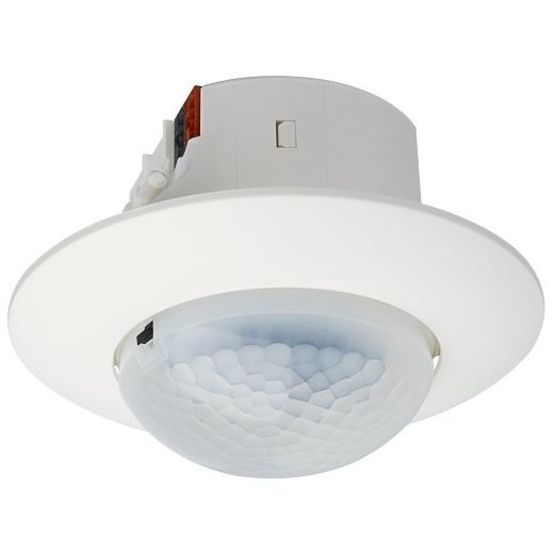
\includegraphics[width=\textwidth,height=.15\textheight,keepaspectratio]{images/detecteurPresence}

  \UPSTIaCompleter{\large{Capteur logique}}

\end{minipage}
\begin{minipage}[b]{0.24\textwidth}
\centering
  Barrière infrarouge
  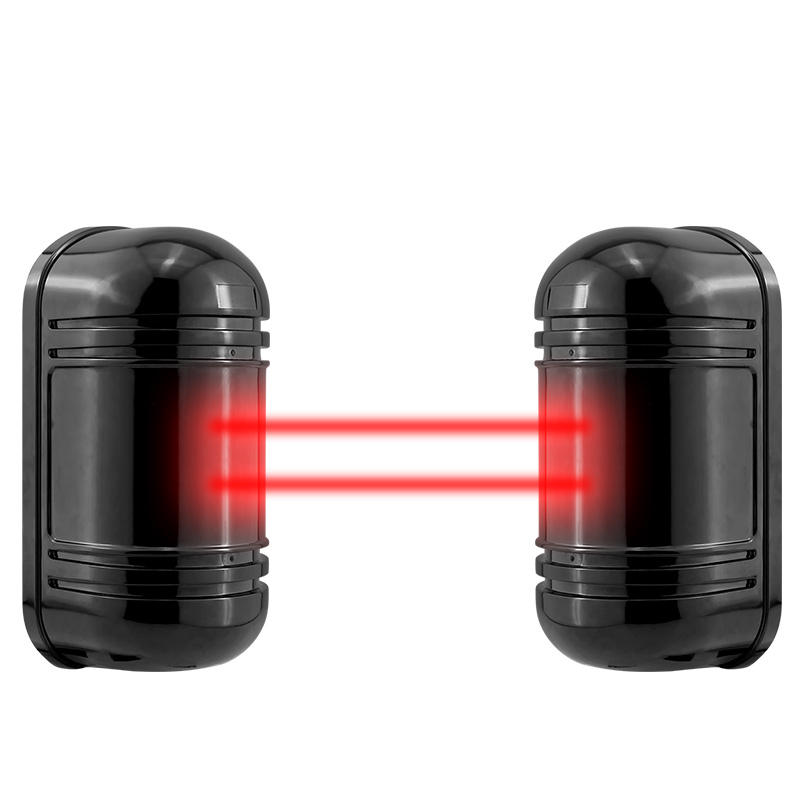
\includegraphics[width=\textwidth,height=.15\textheight,keepaspectratio]{images/barriereInfrarouge}

  \UPSTIaCompleter{\large{Capteur logique}}

\end{minipage}
\begin{minipage}[b]{0.24\textwidth}
\centering
  Haut parleur
  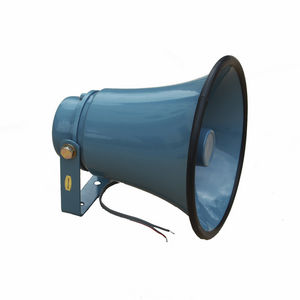
\includegraphics[width=\textwidth,height=.15\textheight,keepaspectratio]{images/hautParleur}

  \UPSTIaCompleter{\large{Actionneur}}

\end{minipage}

\UPSTIquestion{Dessiner un signal en sortie d'un capteur analogique.}

\UPSTIquadrillage{4}

\UPSTIquestion{Dessiner un signal en sortie d'un capteur numérique.}

\UPSTIquadrillage{3}

\end{UPSTIactivite}
